\section{Discretization}

The conservation laws presented in the previous section will now be converted into a set of nonlinear, algebraic equations whose solution represents the system's evolution in space-time.
In general, the purpose of this \textit{discretization} is to transform the problem from finding a set of functions that have a defined value for every point of space-time to finding a set of unknown coefficients to chosen functions which represent the solution over a discrete subset of space-time.
The motivation behind this conversion is that finding a vector of unknowns to balance a set of algebraic equations is easier, though still not trivial, than finding a continuous solution to a general, nonlinear differential equation.
Of course, this process adds \textit{discretization errors} to the obtained solution \cite{leveque_finite_2007}; however, those errors are viewed as a necessary cost to effect a useful solution.
Additionally, when the discretization is made carefully, it does not often undermine the underlying physical significance of the conservation laws.

The discussion of discretization is presented in two parts: choice of spatial discretization and choice of temporal discretization.
This separation of concerns is achieved via the \textit{method of lines}, also known as a \textit{semi-discrete scheme}.
The method of lines involves the discretization of the spatial dimension only, such that the system of equations becomes a system of coupled, ordinary differential equations.
The system can then be solved using a standard and robust \Acro{ODE} time integration method \cite{schiesser_numerical_2012}.

It is noted that most of the following discussion assumes the solution being found is one to a differential equation.
As stated in the previous section, the conversion between differential and integral equations is valid as long as the solution has finite values of all required derivatives at every point in the domain.
Because the topic of shockwaves is deemed beyond the scope of this work, the two forms are treated synonymously with a focus on the differential side since that is from where most of the relevant theory is acquired.


\subsection{Spatial Discretization}

The spatial discretization of a system of equations is taken to be both a concrete specification of how the solution is taken to vary in space and how the spatial domain of the system is partitioned.
The first specification concerns what is called the \emph{construction} of the solution, and the second concerns what is called the \emph{partitioning} of the solution.
For a single equation of unknowns, these choices are inexorably linked.
However, a system of equations allows each of the equations to be partitioned differently despite having the same approximation, and thus the two concerns will be explained separately.


\subsubsection{Construction}

The construction of a solution to a system of differential equations involves the explicit selection of a functional form made to balance the system.
Since the actual functional form of the solution is unknown globally, local functional forms of the solution with a varying number of undetermined coefficients (i.e., degrees of freedom) are assumed over a set of discrete points or sections of the domain.
The coefficients are then calculated by requiring the functional forms to balance the system of equations in some manner and satisfy any compulsory compatibility conditions (such as global continuity).
The union of these local functional forms with the determined coefficients then form the approximate global solution.

From that very general framework, there are three often-used methods of construction: finite difference, finite volume, and finite element.
In brief, the main ideas behind these methods are:
\begin{itemize}[topsep=-0.5\parskip]
    %
    %
    \item{A \Acro{FDM} is derived from either local truncated Taylor expansions to approximate derivatives or from local polynomial interpolants with sufficient support\footnote{In this instance, \emph{support} means that the degree of the interpolating polynomial at least matches the differential order of the system such that all polynomial derivatives have non-trivial terms.  For example, a third order differential equation requires a cubic interpolant because any lower degree polynomial would have a third derivative of $0$ and could in no way balance (i.e., support) the differential equation.} for the system being solved. The system is then required to be balanced at every point about which the construction is made.}
    %
    %
    \item{A \Acro{FVM} assumes the global solution to be a collection of disjoint partitions that only communicate at their boundaries via fluxes and are locally defined by an arbitrary polynomial. The equation is then required to be satisfied in an integral-sense over each of the partitions.}
    %
    %
    \item{A \Acro{FEM} assumes the global solution to be a collection of contiguous partitions locally defined by an arbitrary polynomial. The equation is then required to be satisfied in a weighted integral-sense over the entire domain.}
    %
    %
\end{itemize}
 
Finite differences are the oldest class of methods and easily allow for high-order approximations but are not easily extended to non-rectangular grids and may not exactly conserve quantities by construction.
Finite volumes are easily extended to arbitrary grids due to their integral nature and can be guaranteed to ensure exact conservation but arbitrarily high-order approximations are difficult to form.
Finite elements are easily extended to arbitrary grids due to their integral nature and are easily extended to arbitrarily high-order approximations but the global nature of the solution does not necessarily guarantee local conservation of quantities \cite{zienkiewicz_finite_2013}.

The method of approximation used for the remainder of this work will be \Acro{FVM}.
The benefits of arbitrary geometry and exact conservation outweigh the lack of easy high-order methods.
Further, only a first-order method will be pursued and concretely presented in the following section.
Although first-order finite volume methods are known to be diffusive for source-less conservation laws, the method is always stable, even in the presence of shockwaves, and gives order-of-magnitude answers, as those sought in engineering level modeling.
The latter assertion is demonstrated in the following example.

Consider numerically solving the following one-dimensional boundary value problem:
\begin{equation}
    \deriv{T}{x}{2} = \frac{-\pi^2}{4}\,\Cos\left(\frac{\pi x}{2}\right);\quad\quad T(-1) = 0\,,\quad T(1) = \frac{1}{2}
    \label{Eqn:NM_Example_BVP}
\end{equation}
For all three methods, the $x$ dimension is divided by $n+1$ equidistant points between $-1$ and $1$ with $n$ internal partitions of width $\Delta{x}$.
The algebraic equations from three different approximation methods are derived as follows:
\begin{itemize}
    %
    %
	\item{
        Approximating the unknown $T(x)$ at the $i$-th point by a quadratic polynomial defined by the values of T(x) at the points $x_{i-1}$, $x_{i}$, and $x_{i+1}$, the point-wise enforced finite difference equation is
        \begin{equation}
            \frac{T_{i+1} - 2 T_i + T_{i-1}}{\Delta{x}^2} = \frac{-\pi^2}{4}\,\Cos\left(\frac{\pi x_i}{2}\right).
        \end{equation}
    }
    %
    %
    \item{
        Approximating the value of $T(x)$ over the $j$-th partition between $x_{i-1}$ and $x_{i}$ as a constant value $\bar{T}_{j}$, the partition-wise enforced finite volume equation is
        \begin{equation}
            \deriv{\bar{T}}{x}\bigg\rvert_{i} - \deriv{\bar{T}}{x}\bigg\rvert_{i-1} = 
            \frac{\bar{T}_{j+1} - 2 \bar{T}_j + \bar{T}_{j-1}}{\Delta{x}} = \frac{-\pi^2}{4}\,\Cos\left(\frac{\pi}{2}\,\frac{(x_{i-1}+x_i)}{2}\right) \Delta{x}.
        \end{equation}
        The first expression emphasizes that the finite volume method integrates once to create flux-based difference equations.
        The fluxes are then formed using a chosen relationship between partition values, and the original right-hand is integrated in some approximate fashion over the partition.  The choices leading to the second and third expressions are a piece-wise linear relationship between partition values and the mid-point integration rule for the right-hand side.
    }
    %
    %`
    \item{
        Assuming the unknown $T(x)$ to behave linearly within the two partitions bounded by $x_{i-1}$ and $x_{i+1}$, the partition-wise enforced finite element equation is
        \begin{equation}
            \frac{T_{i+1} - 2 T_i + T_{i-1}}{\Delta{x}^2} = \frac{4}{\Delta{x}^2}\,\Cos\left(\frac{\pi x_i}{2}\right)\,\Sin^2\left(\frac{\pi x_i}{4}\right),
        \end{equation}
        where the right-hand side was integrated exactly over the partitions.
    }
\end{itemize}

The approximate and analytical solutions are shown in \cref{Fig:NM_Example_ApproximationComparison}.
As can be seen, despite the extremely similar difference equations between the three methods, the underlying choice of construction leads to very different approximate solutions.
Furthermore, as seen in \cref{Fig:NM_Example_ApproximationComparisonError}, the FVM's assumption of partition-wise constant data leads to a first-order convergent method instead of the second-order convergence shown by FDM and FEM.
However, regardless of its first-order nature, the solution provided by FVM still qualitatively reproduces the analytical solution.
And because the end goal of this work is not a rigorous resolution of the spatial domain at all scales but a conservative, system-integrated stability analysis, the first-order FVM method is viewed as the best compromise between the FDM and FEM methodologies.


\begin{figure}%
    \centering
    \caption{Solutions of \cref{Eqn:NM_Example_BVP} for the approximation methods discussed using six partitions.}
    \label{Fig:NM_Example_ApproximationComparison}
    \tikzsetnextfilename{Section-Discretization_ExampleConductionValue}
    \IncludeSection{Section-Discretization_ExampleConductionValue.tikz}%
\end{figure}
\begin{figure}%
    \centering
    \caption{L\subs[\;]{2} norm error plots versus partition count. FEM and FDM exhibit second order convergence; FVM exhibits first order.}%
    \label{Fig:NM_Example_ApproximationComparisonError}
    \tikzsetnextfilename{Section-Discretization_ExampleConductionError}
    \IncludeSection{Section-Discretization_ExampleConductionError.tikz}%
\end{figure}


\subsubsection{Partitioning}

Partitioning, alternatively known as \textit{meshing}, involves selecting a collection of partitions whose union recreates the problem geometry as closely as possible.
In general, the partitioning is not unique and may be vary between equations in the system.
For FVM, partitions are commonly referred to as \textit{control volumes}.
Control volumes can be any shape needed to cover the physical domain but, for simplicity, are often limited to polyhedra or a natural differential element in the coordinate system being used.

This work will make use control volumes with completely flat bounding faces.
The flat bounding faces make approximating the surface integrals in the conservation laws more straightforward.
While this may appear limiting, evaluation of the surface integral is only performed where there is a non-zero flux of a conserved quantity.
And since the velocity is assumed to be zero on all solid surfaces within the model assuming no-slip and impermeability, the control volumes can be deformed to fit the bounding physical surface with only the artificial flux exchange surfaces required to be flat.

Additionally, this work employs a so-called \textit{staggered scheme} with two different partitionings: one for the conservation of energy and mass and another for the conservation of bulk momentum.
The staggered scheme overcomes a problem introduced by solving a single, bulk momentum equation: the control volumes used to solve the bulk momentum equation have an inherent flow direction $z_i$, but the mass and energy control volumes are exposed to fluxes of material from any direction.


If the partitionings were the same for all equations, more approximations would need to be introduced to calculate the surface velocities not to mention the burden of having to define an exchange scheme for branching flows.
To exemplify that point, consider \cref{Figure:Branching}.
The dominant flow directions, indicated with red arrows, are all apparent aside from the partition where the flow splits in two.
\begin{figure}[t]%
    \centering
    \caption{A simple, two-dimensional partition diagram of a tee-branch; red arrows indicate a dominant flow direction.}%
    \label{Figure:Branching}%
    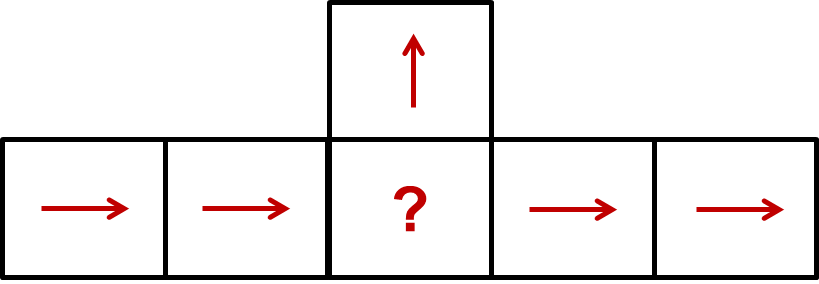
\includegraphics[height=1in]{BranchingProblem.png}%
\end{figure}
If the momentum equations were partitioned on the same grid as the mass and energy equations, the flexibility of the code to model real world situations would be greatly limited.
This single choice of partition is to be contrasted with the one shown in \cref{Figure:TwoPartition}.
By off-setting the center points of the momentum equation's partition, velocities at any direction are able to be calculated as long as the boundaries of the partitions are adjusted appropriately.

Furthermore, the values of the partition-wise constant momentum maybe taken to exist directly at the bounding face of the control volumes.
If chosen in this manner, then the surface flux values for the mass and energy conservation equations have a known advection velocity.
This choice is similar to selecting a single location within an integration rectangle and using the value of the function at that point multiplied by the rectangle's width to approximate the integral.

\begin{figure}[b]%
    \caption{A staggered, two-dimensional diagram of a tee-branch.}
    \label{Figure:TwoPartition}
    \begin{subfigure}[t]{0.49\textwidth}%
        \centering
        \caption{Mass and Energy Partition}%
        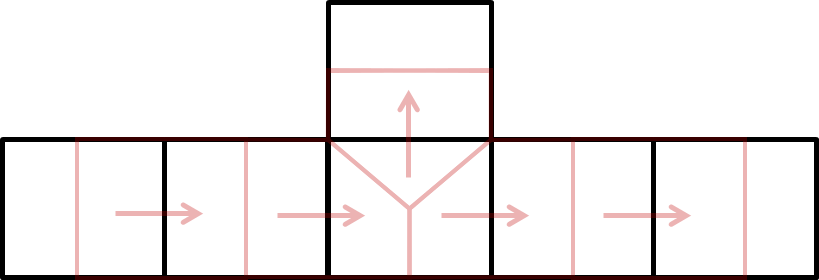
\includegraphics[width=0.98\textwidth]{Staggered_Control.png}%
    \end{subfigure}
    \hfill
    \begin{subfigure}[t]{0.49\textwidth}%
        \centering
        \caption{Momentum Partition}%
        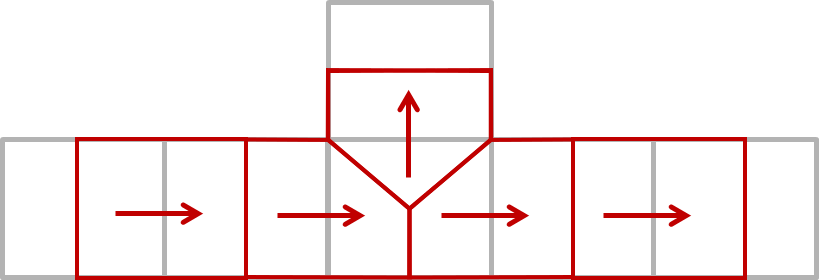
\includegraphics[width=0.98\textwidth]{Staggered_Momentum.png}%
    \end{subfigure}
\end{figure}





\subsubsection{Semi-discrete Conservation Laws}
Using the partition-wise constant constructions and staggered scheme from the previous section, the semi-discrete form of the equations will now be presented.
For efficiency, some terminology will be discussed first.
The system of ordinary differential equations will then be given.

For any model, the spatial domain is partitioned into discrete \textit{control volumes} that will hold the mass and energy of the system.
In order to create a connection between two control volumes through which mass may transfer, identification numbers are used to form a ``from'' and ``to'' relationship between the control volumes; this ``from'' and ``to'' connection creates a partition for the momentum equation called a \textit{momentum cell}.
The connection also carries the bulk flow direction information and forms an exchange surface between the control volumes that is orthogonal to the dominant flow direction.
Lastly, each surface shared by two momentum cells between which momentum may be transferred are called \textit{interfaces}.
For each interface, an ``upwind'' and a ``downwind'' momentum cell must be specified along with the interfaces unit normal, which is assumed to point away from the upwind cell.

\begin{figure}[b]%
    \caption{A staggered, two-dimensional diagram of a tee-branch with identification numbers and interface normals.}
    \label{Figure:Numbered}
    \begin{subfigure}[t]{0.49\textwidth}%
        \centering
        \caption{Mass and Energy Partition}%
    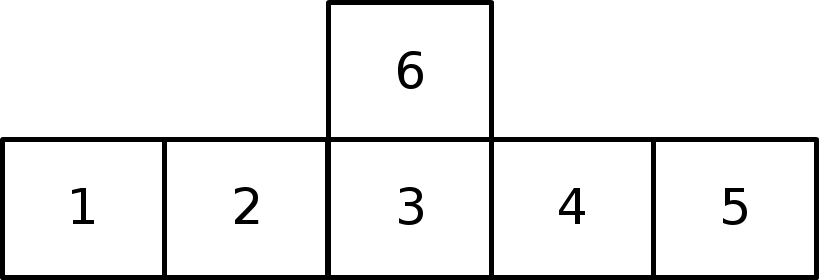
\includegraphics[width=0.95\textwidth]{Staggered_Control-Numbered.png}%
    \end{subfigure}
    \hfill
    \begin{subfigure}[t]{0.49\textwidth}%
        \centering
        \caption{Momentum Partition}%
    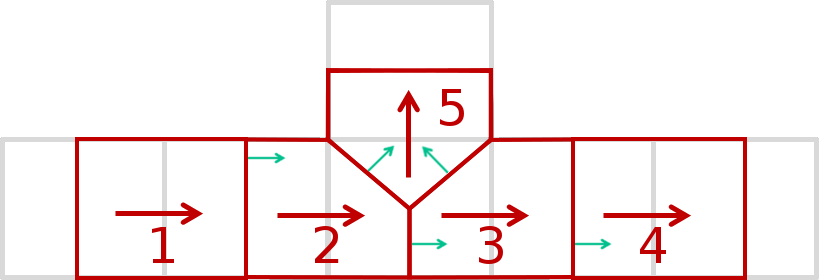
\includegraphics[width=0.95\textwidth]{Staggered_Momentum-NumberedWNormals.png}%
    \end{subfigure}
\end{figure}

The creation of the connections is programmatically done with identification numbers associated with the control volumes and all other numbers induced by those connections.
A physical diagram with identification numbers is shown in \cref{Figure:Numbered}.
The connection information is shown in \cref{Table:Connections}.
These physical connections, flow directions, flow areas, and volumes give enough information to form the semi-discrete form of the equations.



The spatially discretized mass equation for the $k$-th control volume has the form
\begin{equation}
    \deriv{}{t}\!\IntV \rho_k \dV = s^\rho_k V_k + \sum_{n=1}^{N} u_n \rho_{d,n} A_n  \label{Eqn:SemiMass}
\end{equation}
where $s^\rho_k$ is a source term, $V_k$ is the volume of the control volume, $u_n$ is the exchange velocity, $\rho_{d,n}$ is the donor density, and $A_n$ is the exchange surface area.  The index $n$ runs from $1$ to however many other control volumes are connected to $k$.
The donor density $\rho_{d,n}$ is the density of the ``from'' volume if $\Sign(u_n)$ is positive or the density of the ``to'' volume otherwise.
This donor approach ensures exact conservation of mass.

The spatially discretized energy equation for the $k$-th control volume has the form
\begin{equation}
    \deriv{}{t}\! \IntV \rho i_k \dV = s^e_k V_k + \sum_{n=1}^{N} u_n \rho{h}_{d,n} A_n \label{Eqn:SemiEnergy}
\end{equation}
where $s^e_k$ is a source term, $V_k$ is the volume of the control volume, $u_n$ is the exchange velocity, $\rho{h}_{d,n}$ is the donor enthalpy, and $A_n$ is the exchange surface area.  The donor enthalpy $\rho{h}_{d,n}$ is equal to $\rho{i}_{d,n} + P_{d,n}$ is the enthalpy of the ``from'' volume if $\Sign(u_n)$ is positive or the density of the ``to'' volume otherwise.
This donor approach ensures exact conservation of energy.



The spatially discretized momentum equation for the $k$-th momentum cell has the form
\begin{equation}
    \deriv{}{t}\! \IntV \rho u_k \dV = 
    (\rho_k g_k + s^u_k)\,V_k 
    - \sum_{n=1}^{N}   (P_n z_n +  u_{\text{\textsc{i}},n} \rho{u}_{d,n}) A_n 
    - \frac{1}{2} f\subs{\textsc{d},k}\,\frac{L\subs{char,k}}{D\subs{eff,k}}\,\Abs(\rho{u}_k) u_k A_k  \label{Eqn:SemiMomentum}
\end{equation}
where $\rho_k$ is the average mass density of the control volumes spanned by the $k$-th momentum cell, $g_k$ is the dot product of gravity with the dominant flow direction of the cell, $s^u_k$ is the source, $V_k$ is the volume of the cell, $P_n$ is the pressure along the $n$-th interface, $z_n$ is the dot product of the interface's unit normal with the dominant flow direction, $u_{\text{\textsc{i}},n}$ is the interface exchange velocity,
$\rho{u}_{d,n}$ is the donor momentum, $A_n$ is the area of the interface, 
$f$ is the friction factor, $L$ is the friction exchange length, $D$ is the effective diameter, 
$\rho{u}_k$ is the intensive bulk momentum, $u_k$ is the bulk velocity, and $A_k$ is the flow area of the momentum cell.
The interface exchange velocity is a simple average of the upwind and downwind momentums following their dot with the interface normal.
The donor momentum is, as previously done for exact conservation, either the upwind or downwind momentum dependent on the sign of the interface exchange velocity.
All of the intensive quantities are derived from the extensive properties through standard arithmetic relations.


\begin{table}[H]%
    \caption{Summary tables of the connection information used to programmatically construct the example tee-branch.}
    \label{Table:Connections}
    \rowcolors{2}{}{Gray}
    \begin{subtable}[t]{\textwidth}
        \centering
        \caption{From-To Connections}
        \begin{tabular}{cccc}
            \toprule
            From & To & Momentum Cell Number & Dominant Flow Direction \\
            \midrule
            1 & 2 & 1 & $1 \hat{\imath}$ \\
            2 & 2 & 2 & $1 \hat{\imath}$ \\
            3 & 3 & 3 & $1 \hat{\imath}$ \\
            4 & 5 & 4 & $1 \hat{\imath}$ \\
            3 & 6 & 5 & $1 \hat{\jmath}$ \\
            \bottomrule
        \end{tabular}
    \end{subtable}
    \vskip0.8em
    \begin{subtable}[b]{\textwidth}
        \centering
        \caption{Upwind-Downwind Connections}
        \begin{tabular}{cccc}
            \toprule
            Upwind & Downwind & Interface Number & Unit Normal \\
            \midrule
            1 & 2 & 1 & $1 \hat{\imath}$ \\
            2 & 3 & 2 & $1 \hat{\imath}$ \\
            2 & 5 & 3 & $\tfrac{1}{\sqrt{2}} \hat{\imath} + \tfrac{1}{\sqrt{2}} \hat{\jmath}$ \\
            3 & 4 & 4 & $1 \hat{\imath}$ \\
            3 & 5 & 5 & $-\tfrac{1}{\sqrt{2}} \hat{\imath} + \tfrac{1}{\sqrt{2}} \hat{\jmath}$ \\
            \bottomrule
        \end{tabular}
    \end{subtable}
\end{table}


\subsection{Temporal Discretization}

For a model consisting of $N_{\text{\textsc{cv}}}$ control volumes and $N_{\text{\textsc{mc}}}$ momentum cells, \cref{Eqn:SemiMass,Eqn:SemiEnergy,Eqn:SemiMass} constitute a system of $2\,N_{\text{\textsc{cv}}} + N_{\text{\textsc{mc}}}$ ordinary differential equations.
This can be simply expressed as
\begin{equation}
    \deriv{q_i}{t} = f_i(t,q_i).
\end{equation}
In order to turn the above ODE into an algebraic system, another discretization choice must be made.
There are many different types of discretizations to choose from, but this work employs the Implicit Euler Method.
This method was chosen because it is an extremely stable, first-order method that does not necessarily have a restriction on the time-step size for advancement of the equations.
Although, a small time-step is used in practice for accuracy and quick solution of the system.

The Implicit Euler Method approximates the left-hand time derivative as a first-order finite difference and evaluates the right-hand side at the next time-step value:
\begin{equation}
    \frac{q^{p+1}_i - q^p_i}{t^{p+1}-t^p} = f_i(t^{p+1},q^{p+1}_i)
\end{equation}
which upon re-arranging yields the residual form:
\begin{equation}
    r_i(t^{p+1},q^{p+1}) =  q^{p+1}_i - q^p_i + (t^{p+1}-t^p) f_i(t^{p+1},q^{p+1}_i).
\end{equation}
The next time-step value $q^{p+1}$ is unknown and must be found by driving the residual function $r_i(t^{p+1},q^{p+1})$ to or near zero.
The manner chosen to solve this nonlinear, algebraic equation is presented in detail in the next section.




